\begin{figure}
\centering
\subfloat{%
\begin{minipage}{0.40\textwidth}
\begin{tikzpicture}[every tree node/.style={draw,circle},
   level distance=1.8cm,sibling distance=0.7cm,
   edge from parent path={(\tikzparentnode) -- (\tikzchildnode)}]
\Tree
[.a
    \edge node[auto=right] {$\alpha$};
    [.b 
       \edge node[midway,left] {$\beta$};
       [.d ]
       \edge node[midway,right] {$\gamma$};
       [.e ]
        ]
    \edge node[auto=left] {$\delta$};
    [.c 
        \edge node[midway,left] {$\epsilon$};
        [.f ]
        \edge node[midway,right] {$\zeta$};
        [.g ]
        ]
]
\end{tikzpicture}
\end{minipage}
}
\subfloat{%
\begin{minipage}{0.40\textwidth}
\begin{equation*}
A =
\bordermatrix{
           & \mathrm{a} & \mathrm{b} & \mathrm{c} & \mathrm{d} & \mathrm{e} & \mathrm{f} & \mathrm{g} \cr
\mathrm{a} & 0          & \alpha     & \delta     & 0          & 0          & 0          & 0          \cr
\mathrm{b} & \alpha     & 0          & 0          & \beta      & \gamma     & 0          & 0          \cr
\mathrm{c} & \delta     & 0          & 0          & 0          & 0          & \epsilon   & \zeta      \cr
\mathrm{d} & 0          & \beta      & 0          & 0          & 0          & 0          & 0          \cr
\mathrm{e} & 0          & \gamma     & 0          & 0          & 0          & 0          & 0          \cr
\mathrm{f} & 0          & 0          & \epsilon   & 0          & 0          & 0          & 0          \cr
\mathrm{g} & 0          & 0          & \zeta      & 0          & 0          & 0          & 0          \cr
}
\end{equation*}
\end{minipage}
}
\caption{Construction of the graph adjacency matrix for a phylogenetic tree.}
\label{FP_adjacency}
\end{figure}